\chapter{\heiti 调用接口程序}
\section{Python \heiti{接口程序}}
我司为用户提供了Python接口程序。用户可调用接口程序中的函数自己编程生成方波序列与Counter序列,并将其下载到硬件中然后控制仪器播放生成的方波序列以及读回计数结果。使用Python接口程序中的函数时可以参考我司为用户提供的“DDR3\_USB\_8chn\_ccounter\_dll.py”文件中的调用方式。现将用户所需的函数列出,并加以解释。注意在调用接口程序中的函数时,定义的单个方波序列高低电平时间必须在5 ns至2.6 s之间,且必须是0.05 ns的整数倍。定义的单个Counter序列高低电平时间必须在5 ns至5000 s之间,且必须是5 ns的整数倍。
\vspace{0.4cm}

\noindent\fontsize{12pt}{\baselineskip}\textbf{\heiti{函数}PB\_type\_program(pulse)}

传入参数“pulse”是一个列表(list\_0),列表中的每个元素仍然是一个列表(list\_1),每个元素均形如[‘01010101’, 0, 0, 20.0]。list\_1中的第一个元素为一个字符串,字符串由8个‘0’或‘1’组成,从左往右依次代表8个输出通道,‘0’代表该通道输出低电平,‘1’代表该通道输出高电平。list\_1中的第二和第三个元素没有意义,为0即可。list\_1中的第四个元素代表该方波序列状态的持续时间,单位为纳秒。如用户想要在OUT1通道输出一个高电平时间长度为60ns低电平时间为40.05 ns的方波序列,则用户可以令pulse=[[‘10000000’,0,0,60], [‘00000000’,0,0,40.05]],然后调用PB\_type\_program(pulse)即可将该方波序列下载到硬件中。
\vspace{0.4cm}

\noindent\fontsize{12pt}{\baselineskip}\textbf{\heiti{函数}Counter\_program(pulse)}

传入参数“pulse”是一个列表(list\_2),列表中的每个元素仍然是一个列表(list\_3),每个元素均形如[‘1’,0,0,10.0]。list\_3中的第一个元素为‘0’或‘1’,‘0’代表Counter序列为低电平,‘1’代表Counter序列为高电平。list\_3中的第二和第三个元素没有意义,为0即可。list\_3中的第四个元素代表该Counter序列状态的持续时间,单位为纳秒。如用户想要生成一个高电平时间为20ns,低电平时间为15 ns的Counter序列,则用户可以令pulse=[[‘1’,0,0,20], [‘0’,0,0,15]],然后调用Counter\_program(pulse)即可将该Counter序列下载到硬件中。

\newpage
\noindent\fontsize{12pt}{\baselineskip}\textbf{\heiti{函数}start()}

函数没有传入参数,在调用PB\_type\_program( )与Counter\_program( )后,再调用start( )即可向硬件发送指令使仪器开始播放方波序列以及开始计数。
\vspace{0.4cm}

\noindent\fontsize{12pt}{\baselineskip}\textbf{\heiti{函数}stop()}

此函数没有传入参数,用来向硬件发送指令,使仪器停止播放方波,并停止计数。在调用stop( )之后再次调用start( )可以重新使仪器播放方波序列并开始计数。
\vspace{0.4cm}

\noindent\fontsize{12pt}{\baselineskip}\textbf{\heiti{函数}get\_default\_count()}

此函数没有传入参数,可直接调用获得连续计数结果。
\vspace{0.4cm}

\noindent\fontsize{12pt}{\baselineskip}\textbf{\heiti{函数}get\_all\_count()}

此函数没有传入参数,可以直接调用获得计数结果。
\vspace{0.4cm}

\noindent\fontsize{12pt}{\baselineskip}\textbf{\heiti{完整调用过程举例}}

pulse = [[`10000000',0,0,60],[`00000000',0,0,40.05]]\qquad \#  定义方波序列

counter\_pulse = [[`1',0,0,60], [`0',0,0,15] ]\qquad           \#  定义Counter序列

PB\_type\_program(pulse)\qquad            \#  下载方波序列

Counter\_program(counter\_pulse)\qquad     \#  下载方波序列

Start( )\qquad          \#  开始播放序列并开始计数

Continuous\_counter\_result = get\_default\_count()\qquad    \#  获得连续计数结果

Counter\_result = get\_all\_count()\qquad                  \#  获得计数结果

Stop( )\qquad     \#  停止播放序列并停止计数,仅在需要停止播放或计数时使用

\section{C\heiti 接口程序}
我司为用户提供了C接口程序。用户可调用接口程序中的函数自己编程生成方波序列与Counter序列,并将其下载到硬件中然后控制仪器播放生成的方波序列以及读回计数结果。现将用户所需的函数列出,并作出解释。注意在调用接口程序中的函数时,定义的单个方波序列高低电平时间必须在5 ns至2.6 s之间,且必须是0.05 ns的整数倍。定义的单个Counter序列高低电平时间必须在5 ns至5000 s之间,且必须是5 ns的整数倍。

\newpage
\noindent\fontsize{12pt}{\baselineskip}\textbf{\heiti{函数}asg\_program\_all(char **flags,double *time\_length,unsigned long cmd\_num,\\unsigned char **buf,int *buf\_length)}
\begin{table}[H]
\Large
%\caption{}
\begin{tabular}{|m{7cm}<{\centering}|m{7cm}|}
\hline
传入参数 & \makebox[7cm][c]{参数描述} \\ \hline
char **flags & 参数“flags”是一个二维数组,每个元素均为形如“01011010”的字符串。字符串个数代表方波数据的个数,字符串中的‘0’或‘1’从左往右依次代表8个方波输出通道的的状态。‘0’代表低电平,‘1’代表高电平。\\ \hline
double *time\_length & 参数“time\_length”是一个double型一维数组。每个元素代表相应每个方波序列状态的时间长度,单位为纳秒。该数组长度必须与“flags”的数组长度相同。 \\\hline
unsigned long cmd\_num & 参数“cmd\_num”是一个正整数,表示方波序列数据的个数。 \\\hline
unsigned char **buf & 参数“buf”是一个二维空字符数组。即每个元素为一空字符串,字符串的个数为8,每个字符串的长为cmd\_num的10倍。 \\\hline
int *buf\_length & 参数“buf\_length”必须是\{0,0,0,0,0,0,0,0\}。 \\\hline
\end{tabular}
\end{table}

\newpage
\noindent\fontsize{12pt}{\baselineskip}\textbf{\heiti{函数}asg\_counter\_program\_all(char **flags, double *time\_length, unsigned long cmd\_num, unsigned char **buf,int *buf\_length)}
\begin{table}[H]
\Large
%\caption{}
\begin{tabular}{|m{7cm}<{\centering}|m{7cm}|}
\hline
传入参数 & \makebox[7cm][c]{参数描述} \\ \hline
char **flags & 参数“flags”是一个二维数组,即每个元素均为形如“0”的字符串。字符串的个数代表方波的个数,字符串中的‘0’或‘1’代表Counter序列的状态,‘0’代表低电平,‘1’代表高电平。\\ \hline
double *time\_length & 参数“time\_length”是一个double型数组。每个元素代表相应每个Counter序列状态的时间长度,单位为纳秒。该数组长度必须与“flags”的数组长度相同。\\\hline
unsigned long cmd\_num & 参数“cmd\_num”是一个正整数,表示Counter序列数据的个数。 \\\hline
unsigned char **buf & 参数“buf”是一个二维空字符数组。即每个元素为一空字符串,字符串的个数为1,每个字符串的长为cmd\_num的10倍。\\\hline
int *buf\_length & 参数“buf\_length”必须是\{0\}。 \\\hline
\end{tabular}
\end{table}
\vspace{0.4cm}

\noindent\fontsize{12pt}{\baselineskip}\textbf{\heiti{函数}asg\_start( )}

此函数没有传入参数,调用asg\_program\_all( )与asg\_counter\_program\_all( )后,再调用asg\_start( )即可向硬件发送指令使仪器开始播放方波序列以及开始计数。

\newpage
\noindent\fontsize{12pt}{\baselineskip}\textbf{\heiti{函数}asg\_stop( )}

 此函数没有传入参数,用来向硬件发送指令,使仪器停止播放方波,并停止计数。在调用asg\_stop( )之后再次调用asg\_start( )可以重新使仪器播放方波序列并开始计数。

\section{\heiti 两种接口程序比较}

现将Python接口程序与C接口程序中用户需要调用的函数做一对比,方便用户更好的理解调用接口程序的过程。
\begin{table}[H]
\Large
%\caption{}
\begin{tabular}{|m{1.5cm}<{\centering}|m{5cm}|m{6.5cm}|}
\hline
接口程序 & \makebox[6cm][c]{Python} & \makebox[6.5cm][c]{C}\\ \hline
\vspace{5cm}\multirow{4}{1in}{函数名} & PB\_type\_program(pulse),将方波数据下载到硬件中。& asg\_program\_all(char **flags, double *time\_length, unsigned long cmd\_num, unsigned char **buf, int *buf\_length),将方波数据下载到硬件中。\\\cline{2-3}
&Counter\_program(pulse),将Counter序列数据下载到硬件中。& asg\_counter\_program\_all(char **flags, double *time\_length, unsigned long cmd\_num, unsigned char **buf, int *buf\_length),将Counter序列数据下载到硬件中。\\\cline{2-3}
&start( ),开始播放方波并开始计数。& asg\_start( ),开始播放方波并开始计数。\\\cline{2-3}
&stop( )停,止播放方波并停止计数。& asg\_stop( ),停止播放方波并停止计数。\\
\hline
\end{tabular}
\end{table}
%\begin{figure}
%\centering
%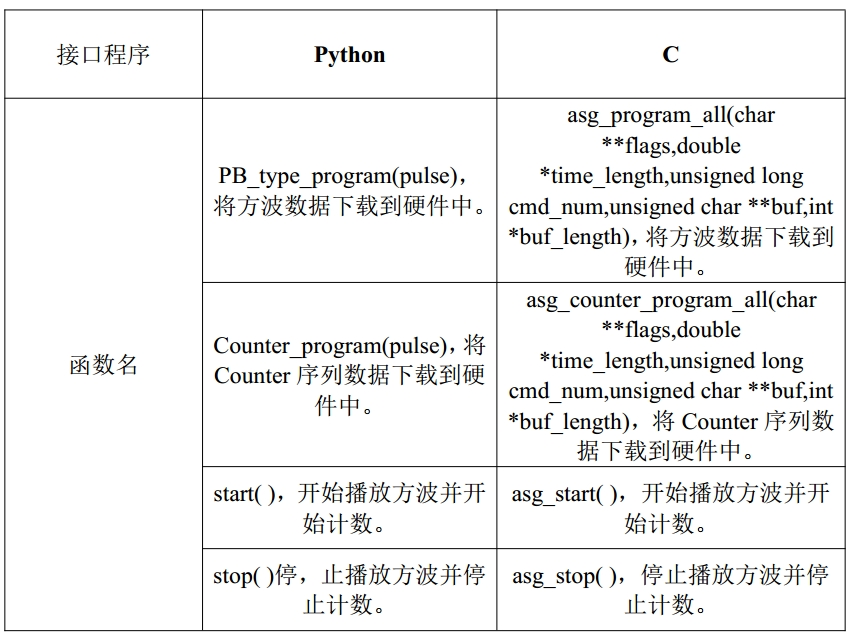
\includegraphics[width=16cm]{last_table}
%\end{figure}
